\documentclass{sigkddExp}
\usepackage{graphicx}
\usepackage{url}
\usepackage{booktabs}
\usepackage{times}
\pdfpagewidth=8.5in
\pdfpageheight=11in
\pagestyle{empty}
\emergencystretch=2em
\tolerance=2000
\begin{document}
\title{Housing Price Prediction with Regression and Feature Importance Analysis}
\numberofauthors{1}
\author{\alignauthor Makungu Ndlovu\\
\affaddr{University of Pretoria}\\
\affaddr{COS802 Project Report}\\
\affaddr{Student number 16153970}}
\maketitle
\begin{abstract}
Housing valuation requires predictions that account for property characteristics while making error patterns and model behaviour understandable. This project compares linear regression, Ridge regression, random forests and XGBoost on 2,930 residential sales in Ames, Iowa. A fixed split reserves 586 sales for final testing; five-fold cross-validation on the remaining 2,344 sales supports model selection. The study compares original predictors with a representation adding ten domain-informed features, including total floor area and a quality-by-living-area interaction. Engineered XGBoost achieved the lowest development RMSE of \$22,195 and a held-out MAE of \$13,885, RMSE of \$25,354 and $R^2$ of 0.900. The engineered pipeline reduced XGBoost development RMSE by 1.95\%, whereas linear and Ridge RMSE increased. The comparison also differs in structural-missingness treatment, so it does not isolate feature addition alone. A separate fixed-configuration ablation found a 4.35\% RMSE increase when both dominant engineered features were removed. SHAP identified the quality-area interaction as the strongest contributor, but expensive properties remained difficult to predict. The contribution is a reproducible comparative analysis with explicit validation boundaries, feature sensitivity and error diagnosis, rather than a new regression algorithm or a deployment-ready valuation service.
\end{abstract}

\section{Introduction}
Residential properties differ in size, condition, age, amenities and location. A useful price estimate must combine these attributes rather than rely on a single average price or floor-area rule. At the same time, an attractive overall score can conceal large errors on unusual houses. A predictive study should therefore examine both how well a model performs and where its estimates become unreliable.

This project treats housing valuation as supervised regression. Given structured property attributes $x$, the objective is to estimate the observed sale price $y$ in US dollars. The study uses the Ames Housing data introduced by De Cock~\cite{decock}. The prediction target is the recorded transaction price, not an independently observed intrinsic value. The scope is historical sales from one city; no claim is made about current South African property prices or future market forecasting.

The central question is whether domain-informed representations improve prediction beyond the original attributes, and whether their predictive usefulness is consistent across model families. Four research questions guide the experiments:
\begin{enumerate}
\item How accurately can prices be predicted from the original structured predictors relative to a mean-price baseline?
\item How does adding domain-informed features affect predictive performance?
\item How do linear, regularised linear, bagging-based and boosting-based regressors compare under the same development folds?
\item Which attributes influence the selected model's predictions, and what do its errors reveal about its limitations?
\end{enumerate}

These questions distinguish model choice from representation choice. Linear regression offers a simple additive reference, Ridge tests coefficient shrinkage, random forests model nonlinear relationships through averaged trees, and XGBoost builds a sequential tree ensemble. Engineered features provide alternative descriptions of existing information: for example, combining quality and area explicitly may make a useful relationship easier for a restricted learner to represent. Such features do not create new observations or external information.

The empirical contribution has three parts. First, the project compares four regression families using saved folds and training-only fitted preprocessing. Second, it reports both favourable and unfavourable effects of the engineered pipeline. Third, it links global and local SHAP explanations to fixed-configuration ablation and held-out error analysis. The findings support engineered XGBoost for this particular experimental setting, while identifying large-price errors, preprocessing differences and limited external validity as important qualifications.

\section{Background and Related Work}
\subsection{Housing data and valuation studies}
De Cock~\cite{decock} introduced Ames Housing as a substantial, interpretable alternative to the Boston Housing data for regression education. It describes sales from 2006--2010 and contains a mixture of quantitative and categorical property attributes. Its detailed quality, area and amenity variables make it suitable for studying preprocessing and feature engineering. This project uses that public benchmark to investigate a methodological question; it does not claim to introduce a new housing dataset.

Antipov and Pokryshevskaya~\cite{antipov} applied random forests to residential-apartment mass appraisal and proposed segment-based diagnostics for detecting areas of poor prediction or systematic bias. Their results motivate evaluating tree ensembles and examining subgroups rather than relying exclusively on a global error measure. Their apartment market and comparison design differ from Ames, so their numerical performance is not treated as a directly comparable benchmark here.

\subsection{Regression and tree ensembles}
Ordinary least squares estimates an additive relationship between encoded attributes and price. Its simplicity provides an informative reference, but useful nonlinearities and interactions must be represented explicitly. Housing predictors can also be correlated: different area measurements and quality indicators describe overlapping aspects of a property. Ridge regression, introduced by Hoerl and Kennard~\cite{ridge}, adds a coefficient penalty to stabilise estimation in the presence of such dependence. Shrinkage can improve prediction, but does not guarantee that adding predictors will reduce every error metric.

Breiman's random forests~\cite{breiman} combine randomised decision trees. For regression, averaging their predictions can reduce the instability of individual trees while retaining nonlinear partitions. This provides a different way to represent quality thresholds and interactions from a global linear function. The present experiment varies tree depth, leaf size and feature sampling within a small, documented search.

Chen and Guestrin~\cite{xgboost} describe XGBoost as an efficient, regularised tree-boosting system. Successive trees improve an ensemble objective, while learning rate, depth and regularisation control complexity. This makes XGBoost a relevant candidate for heterogeneous tabular attributes. Its published success does not determine the result on Ames: the project evaluates it against simpler alternatives using the same folds, target scale and primary selection metric.

\subsection{Explanation and evaluation}
Lundberg and Lee~\cite{shap} proposed SHAP as an additive framework that assigns contributions to features for an individual prediction. Aggregating absolute contributions offers a global view of model use, while signed contributions explain particular predictions relative to a reference value. Here, SHAP is used to describe a fitted predictor. A large contribution is neither a causal effect of a renovation nor a guaranteed economic return from changing an attribute.

Cawley and Talbot~\cite{cawley} show that optimising a model-selection criterion can itself overfit finite-sample evaluation estimates. This motivates retaining a separate test set instead of presenting the best tuning score as independent evidence. The project uses cross-validation to select a configuration and reports a frozen held-out estimate separately. Its post-hoc sensitivity analysis is exploratory evidence about representation, not another independent model-selection test.

Taken together, this literature suggests an evaluation that combines a simple reference, nonlinear models, explicit representation comparisons and diagnosis of uneven errors. The project addresses that combination within one reproducible Ames split. It makes no state-of-the-art claim against published Ames studies or competition leaderboards, whose splits, preprocessing and evaluation scales may differ.

\section{Methodology and Models}
\subsection{Dataset and experimental boundary}
The raw project file contains 2,930 rows and 82 columns, including \texttt{SalePrice}. The row-order field \texttt{Order} and parcel identifier \texttt{PID} are excluded, leaving 79 original predictors. Ten derived attributes increase the engineered representation to 89 predictors before encoding. The task uses structured tabular attributes only. Property-description NLP, external geocoding and image features are outside the implemented scope.

The split uses random seed 16153970 and preserves 2,344 development observations and 586 test observations. Target-informed exploration and tuning use development data. Five shuffled folds with saved memberships are reused across configurations, allowing comparisons on the same validation observations. Fold metrics are averaged arithmetically; reported standard deviations describe variation across the five folds, not confidence intervals for population performance.

The final model is fitted on all development observations after selection. Held-out targets are used for final evaluation and subsequent diagnostic descriptions. They are not used to choose a replacement final model. This random holdout estimates performance for sales drawn from the same historical mixture. It is not a forward-in-time or geographically independent validation.

\subsection{Preprocessing and structural absence}
The reusable preprocessing code separates numerical, ordered categorical and nominal variables. Numerical missing values use training-fold medians. Numerical predictors are standardised for linear/Ridge modelling, while tree models use unscaled numerical inputs. Ordered categories use manually specified orderings, with an encoded value of $-1$ for an unseen category. Nominal attributes use one-hot encoding with unseen categories ignored. Remaining categorical gaps use the training-fold most frequent value. These transformations are fitted inside each training fold rather than on all validation data.

The feature-engineering transformer replaces missing entries in a defined set of amenity-related categorical columns with an explicit \texttt{None} category. These include basement, garage, fireplace and pool descriptors. This distinguishes a missing amenity from an unspecified typical category where the recorded absence has that meaning. The assumption is operational rather than infallible: a missing entry caused by incomplete recording could still be mistaken for true absence.

A code audit identified an important comparison boundary. Notebook 04's original arm passes the raw development columns directly to the imputation/encoding pipeline. Its engineered arm first applies the structural-absence transformer as well as adding derived features. Consequently, the principal original-versus-engineered comparison measures a \emph{pipeline change}, not a perfectly controlled feature-addition effect. The linear reference is carried over from Notebook 03. The report retains the recorded results and makes this distinction explicit rather than silently relabelling them as a pure feature experiment.

Notebook 06 offers a more controlled complementary analysis: it starts from the same engineered frame and removes selected derived columns while retaining its structural-absence treatment. This design holds more of the preprocessing constant. However, it is post-hoc and informed by the earlier explanation results, so it should be interpreted as sensitivity evidence rather than pre-registered confirmation.

\subsection{Domain-informed features}
The ten features use only attributes available in the record and require no target-dependent estimation. Their construction is summarised in Table~\ref{tab:features}. Ages are clipped at zero to avoid negative values. Missing components of area and bathroom sums are set to zero. The amenity flags likewise treat missing counts or areas as zero before testing presence. These choices make feature construction deterministic but can understate an attribute when a missing measurement does not mean absence.

\begin{table}[t]
\caption{The ten added features. SF denotes square feet.}
\label{tab:features}
\centering\small
\begin{tabular}{p{0.31\columnwidth}p{0.59\columnwidth}}
\toprule
Feature & Construction \\
\midrule
HouseAge & Sale year minus build year, clipped at zero \\
RemodAge & Sale year minus remodel year, clipped at zero \\
TotalSF & Basement + first-floor + second-floor area \\
TotalBathrooms & Full bathrooms + 0.5 half bathrooms, including basement \\
TotalPorchSF & Open, enclosed, three-season and screen porches + wood deck area \\
HasGarage & Garage area greater than zero \\
HasBasement & Basement area greater than zero \\
HasFireplace & Fireplace count greater than zero \\
HasPool & Pool area greater than zero \\
QualLivArea & Overall quality multiplied by above-ground living area \\
\bottomrule
\end{tabular}
\end{table}

The quality-area interaction expresses the hypothesis that floor area is interpreted differently at different quality levels. Total floor area aggregates related components, while age and amenity indicators provide simpler representations of information already present. Because the component predictors remain in the model, these features are correlated with existing variables. Interpretation must consider this redundancy: a low importance score for a component does not mean that its underlying information is irrelevant.

Validation checks confirm the presence of all engineered fields, finite and nonnegative values where applicable, binary amenity flags, and alignment of development and test feature columns. They check implementation consistency rather than prove that the feature assumptions are economically correct. The source also retains the numeric storage type of \texttt{MS SubClass}; treating this category-like code as numeric is a limitation that merits a controlled future comparison.

\subsection{Models and search design}
The naive baseline predicts the mean price from each training fold. Linear regression estimates coefficients without an explicit shrinkage penalty. Ridge minimises squared residuals with an additional $L_2$ coefficient penalty:
\begin{equation}
\min_{\beta_0,\beta}\ \sum_i(y_i-\beta_0-x_i^\top\beta)^2
    +\alpha\|\beta\|_2^2 .
\end{equation}
The intercept is not included in the penalty. The Ridge search tests $\alpha\in\{0.1,1,10,100\}$. Scaling is important because otherwise penalty strength depends strongly on the units of the numerical predictors.

The random-forest search evaluates four prescribed configurations, all with 400 trees: unrestricted depth with minimum leaf size 1 or 2 and feature fraction 1.0; or depth 20 with leaf size 1 or 2 and feature fraction 0.7. These are four configurations, not a full Cartesian search over every combination. Each tree ensemble uses the project seed.

XGBoost also evaluates four prescribed configurations. The first two use 500 trees, depth 3, row and column fractions 0.8, $\lambda=1$, and learning rates 0.03 and 0.05 respectively. The third uses 400 trees, depth 4, learning rate 0.03, row and column fractions 0.8 and $\lambda=1$. The fourth uses the selected settings described below. The objective is squared-error regression. Together, three tuned families, two representations, four configurations and five folds produce 120 tuning fits. The fixed linear and earlier target-scale baselines are separate from that count.

The selected model is engineered XGBoost with 400 trees, depth 4, learning rate 0.05, row and column subsampling 0.9 and $\lambda=5$. It is trained directly on dollar prices. The baseline experiments also compared raw targets with $\log(1+y)$ and transformed log-model predictions back to dollars. The final selection follows dollar-scale RMSE. Evaluated predictions are clipped below at zero; this constraint is part of the recorded pipeline and should be preserved during reproduction.

\subsection{Evaluation metrics and uncertainty}
For $n$ observations, predictions $\hat y_i$ and residuals $e_i=y_i-\hat y_i$, the primary metric and companion metrics are
\begin{align}
\mathrm{RMSE}&=\sqrt{\frac{1}{n}\sum_{i=1}^n e_i^2},\\
\mathrm{MAE}&=\frac{1}{n}\sum_{i=1}^n |e_i|,\\
R^2&=1-\frac{\sum_i e_i^2}{\sum_i(y_i-\bar y)^2}.
\end{align}
RMSE emphasises large errors and is used consistently for development selection. MAE communicates average absolute dollar error with less emphasis on extreme misses. $R^2$ expresses fit relative to variation around the evaluation-sample mean. It is not a percentage of predictions that are correct. Reporting all three exposes trade-offs that a single score would hide.

The model is not selected using percentage error or RMSLE. Those metrics answer different questions by emphasising relative rather than absolute errors. In particular, neither MAPE nor a ratio between MAE and a group's median price should be substituted for an uncomputed case-level percentage-error metric. Future comparisons could include median absolute percentage error if relative valuation error is a deployment priority.

For held-out uncertainty, 5,000 bootstrap samples resample the 586 paired outcomes and predictions with replacement using seed 16153970. Each sample recomputes the metrics; the 2.5th and 97.5th percentiles form the reported 95\% intervals. The model is not refitted. These intervals therefore describe test-sample uncertainty conditional on the fitted model, not training-procedure variability, market drift or a prediction interval for a new individual house.

\subsection{Interpretability and sensitivity}
TreeExplainer is applied to the final XGBoost model. Global importance is the mean absolute SHAP value for a seeded sample of 300 test observations. Local explanations use the test cases with the lowest, middle-ranked and highest absolute errors. This selection deliberately illustrates different outcomes; the examples are not an independent representative sample. The global statistic measures contribution magnitude and does not by itself establish the direction of an attribute's effect.

The development-only sensitivity analysis preserves the selected hyperparameters and saved folds. It removes the quality-area interaction, total floor area, both together, and all ten derived features. Another variant removes \texttt{Sale Type} and \texttt{Sale Condition}, testing a scenario in which transaction circumstances are unavailable. These fits do not replace the final model. Their relationship to the main experiment must also account for the structural-missingness difference described above.

\section{Experiments and Results}
\subsection{Development comparisons}
The naive mean predictor achieved development RMSE \$79,592 and MAE \$58,315. Table~\ref{tab:cv} shows that all four model families substantially improve on this reference. The best recorded pipeline, engineered XGBoost, reduces mean CV RMSE by approximately 72.1\% relative to the naive predictor. This is a descriptive development comparison, not a separately tested percentage improvement on future sales.

\begin{table}[t]
\caption{Development five-fold results. O = original; E = engineered. RMSE and its fold SD, and MAE, are in USD. Tuned scores are used for selection, not independent final assessment.}
\label{tab:cv}
\centering\small
\begin{tabular}{llrrrr}
\toprule
Model & Rep. & RMSE & SD & MAE & $R^2$\\
\midrule
Linear & O & 30,677 & 6,234 & 17,462 & .845\\
Linear & E & 32,094 & 10,573 & 16,390 & .820\\
Ridge & O & 29,938 & 5,115 & 17,495 & .854\\
Ridge & E & 30,634 & 6,310 & 16,910 & .845\\
Forest & O & 25,909 & 2,399 & 15,472 & .893\\
Forest & E & 25,232 & 2,519 & 15,101 & .898\\
XGBoost & O & 22,636 & 2,740 & 13,880 & .918\\
XGBoost & E & \textbf{22,195} & 3,522 & \textbf{13,516} & \textbf{.922}\\
\bottomrule
\end{tabular}
\end{table}

Among original representations, XGBoost ranks first, followed by random forest, Ridge and linear regression. The same ordering holds for the engineered representations. Engineered XGBoost improves RMSE by \$3,036, or about 12.0\%, relative to engineered random forest. The finding supports boosting within the tested search budget; it does not establish superiority over every possible forest or linear specification.

Figure~\ref{fig:cv} highlights the model-dependent pipeline effect. The engineered version reduces RMSE by 1.95\% for XGBoost and 2.61\% for random forest. In contrast, RMSE rises by 2.32\% for Ridge and 4.62\% for linear regression. Nevertheless, both linear models improve in MAE. For example, linear MAE falls from \$17,462 to \$16,390 while RMSE rises from \$30,677 to \$32,094. This combination is consistent with lower average absolute error accompanied by greater sensitivity to a subset of large errors; aggregate metrics alone do not identify which observations cause the difference.

\begin{figure}[t]
\centering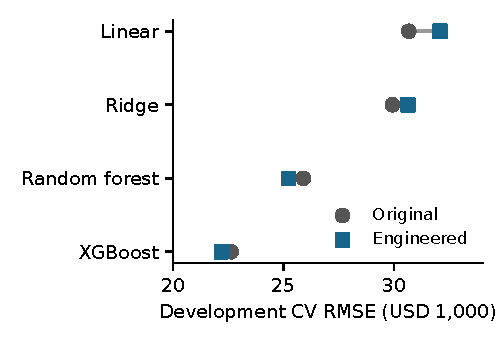
\includegraphics[width=\columnwidth]{figures/cv_comparison.pdf}
\caption{Original and engineered pipeline CV RMSE. Lower is better. The comparison includes structural-missingness changes; it is not a feature-only intervention.}
\label{fig:cv}
\end{figure}

The earlier raw/log target baseline reinforces the importance of the chosen metric. Original Ridge with the fixed baseline settings achieved raw-target RMSE \$30,145, versus \$45,714 after log-target fitting and back-transformation. Its MAE improved from \$17,547 to \$15,378 in the log version. The log model's fold RMSE SD was approximately \$34,968, indicating instability across those folds. These results do not imply that log targets are intrinsically unsuitable; they show that a favourable target distribution or improved MAE does not guarantee lower dollar RMSE under this implementation.

The 1.95\% XGBoost gain is modest relative to fold-to-fold variability. No paired significance test or repeated outer validation supports a claim of statistical significance. Moreover, the best engineered and original XGBoost configurations have different hyperparameters. The main table therefore compares selected pipelines. The next sections separately assess the frozen pipeline's test performance and its response to feature removal.

\subsection{Frozen held-out performance}
Table~\ref{tab:test} reports the final results on the 586 reserved observations. The MAE of \$13,885 provides a direct interpretation of average absolute prediction error. RMSE is substantially larger at \$25,354, showing the influence of large residuals. The $R^2$ of 0.900 indicates that squared error is approximately one tenth of the squared deviations around the test mean; it does not mean that individual prices are predicted with 90\% accuracy.

\begin{table}[t]
\caption{Final engineered-XGBoost performance on 586 held-out sales. Intervals use 5,000 paired test bootstraps without refitting.}
\label{tab:test}
\centering
\begin{tabular}{lrr}
\toprule
Metric & Estimate & 95\% interval\\
\midrule
MAE (USD) & 13,885 & [12,372, 15,772]\\
RMSE (USD) & 25,354 & [18,165, 34,407]\\
$R^2$ & 0.900 & [0.840, 0.941]\\
\bottomrule
\end{tabular}
\end{table}

Test RMSE exceeds the selected CV mean by approximately \$3,159, or 14.2\%. This gap is compatible with a different mix of difficult observations and the optimism associated with selecting the best development score. It is not, by itself, proof of leakage or a precise estimate of overfitting. The broad RMSE interval also cautions against presenting a single point estimate as highly stable.

The bootstrap holds the training outcome fixed and assumes the test rows can be resampled as exchangeable cases. Dependence among nearby or related properties is not modelled by this procedure. Consequently, the interval is narrower in scope than the uncertainty that would accompany deployment in another market or another time period.

\subsection{Residuals and price segments}
Figure~\ref{fig:residual} reproduces the saved residual diagnostic from the final notebook. Residuals are actual minus predicted prices, so positive values indicate underprediction. The plot contains several substantial deviations, including a particularly large positive residual. Aggregate accuracy therefore coexists with individual failures that would matter in an operational valuation setting.

\begin{figure}[t]
\centering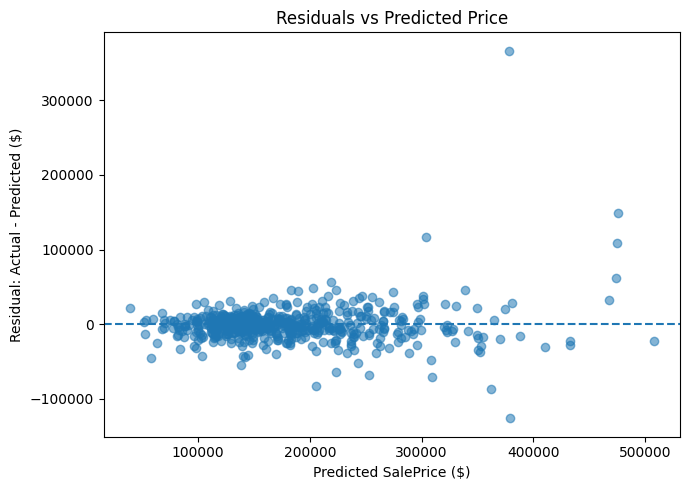
\includegraphics[width=\columnwidth]{figures/residuals.png}
\caption{Saved held-out residual plot from Notebook 05. Large deviations remain despite the favourable aggregate $R^2$. No observations were removed to improve the reported test metrics.}
\label{fig:residual}
\end{figure}

Table~\ref{tab:quartile} groups test observations by actual-price quartile. The highest quartile has MAE \$24,560, more than twice the lowest quartile's \$11,664. Its RMSE is \$43,842, compared with \$16,697 in the lowest quartile. The middle-price groups have smaller absolute errors. These are observed dollar-error differences; they do not establish worse percentage accuracy for expensive houses.

\begin{table}[t]
\caption{Test errors by actual-price quartile, in USD. Mean residual is actual minus predicted. Tied prices produce unequal group sizes.}
\label{tab:quartile}
\centering\small
\begin{tabular}{lrrrr}
\toprule
Quartile & $n$ & MAE & RMSE & Mean residual\\
\midrule
Q1 lowest & 147 & 11,664 & 16,697 & $-7,460$\\
Q2 & 150 & 8,747 & 12,227 & $-327$\\
Q3 & 143 & 10,660 & 15,115 & $-1,922$\\
Q4 highest & 146 & 24,560 & 43,842 & 7,583\\
\bottomrule
\end{tabular}
\end{table}

The mean residuals show overprediction in the lowest group and underprediction in the highest group. This is consistent with predictions being less extreme than observed prices, but the groups are formed using the realised target. Conditioning on actual-price bands can itself produce such patterns. These diagnostics should not be interpreted as a causal explanation or an unbiased calibration test based on predicted-price bands.

The largest-error local example has an actual price of \$745,000 and a prediction of approximately \$378,600, an underprediction of \$366,400. Derived from the stored prediction and overall RMSE, this single case contributes approximately 35.6\% of total test squared error. This helps explain why RMSE and its bootstrap interval are sensitive to rare outcomes. It does not justify removing the case after seeing its error: the reported evaluation retains it, and no evidence in this analysis establishes that the recorded price is erroneous.

\subsection{Global and local explanations}
Figure~\ref{fig:shap} shows the eight largest global mean absolute SHAP values. The quality-area interaction dominates at approximately \$27,896, followed by total floor area at \$6,895 and overall quality at \$5,777. Build year, finished basement area and overall condition also contribute. These are average contribution magnitudes within the 300-case explanation sample, not increases in market price per unit change.

\begin{figure}[t]
\centering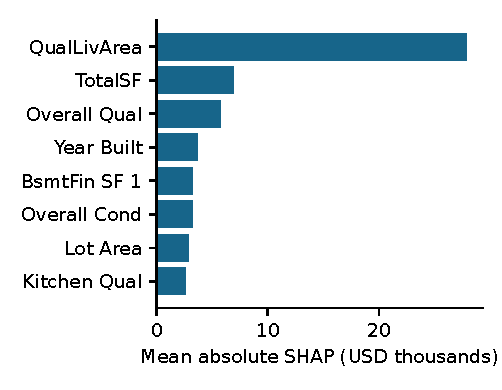
\includegraphics[width=\columnwidth]{figures/shap_importance.pdf}
\caption{Global importance from a seeded sample of 300 test sales. Magnitudes describe the fitted model and depend on its feature representation.}
\label{fig:shap}
\end{figure}

The local examples demonstrate why global ranking alone is incomplete. In the lowest-error example, the actual price is \$105,000 and the prediction is \$104,970. The interaction and total area have negative SHAP contributions of about \$35,736 and \$14,076 relative to the model reference. In the middle-ranked error example, the model predicts \$205,291 for a \$214,000 sale; total area contributes positively by about \$10,098. These selected cases illustrate different signed contributions rather than establish a universal price rule.

In the highest-error example, the interaction contributes about \$105,011 positively, while lot frontage contributes about \$54,791 negatively. Even with a large positive quality-area contribution, the prediction remains far below the recorded \$745,000 sale. A plausible explanation of how a model assembled its estimate is therefore not evidence that the estimate is adequate. The exported local tables show only the ten largest contributions; their sum alone does not reconstruct the full prediction without the baseline and remaining features.

Correlated original and engineered variables complicate interpretation. For example, an interaction can absorb model reliance that might otherwise appear under its components. SHAP does not establish that increasing quality or living area would cause the indicated price change. This is why the project supplements explanations with ablation rather than treating the global ranking as sufficient proof of incremental predictive value.

\subsection{Feature ablation and sale context}
Table~\ref{tab:ablation} summarises the fixed-configuration development sensitivity experiments. Removing the interaction increases RMSE by 2.06\%; removing total floor area increases it by 1.22\%. Removing both increases RMSE by 4.35\%, supporting their joint predictive usefulness for this fitted configuration. Removing all ten features raises RMSE by 3.75\%, less than removing the two together. This non-monotonicity is possible because refitting a tree ensemble changes how the remaining attributes are used; individual feature effects are not additive.

\begin{table}[t]
\caption{Post-hoc development sensitivity with fixed XGBoost settings and five saved folds. Percentage changes use the full engineered baseline.}
\label{tab:ablation}
\centering\small
\begin{tabular}{lrr}
\toprule
Representation & RMSE (USD) & Change\\
\midrule
Full engineered & 22,195 & ---\\
Without QualLivArea & 22,652 & +2.06\%\\
Without TotalSF & 22,467 & +1.22\%\\
Without both & 23,160 & +4.35\%\\
Without all ten & 23,028 & +3.75\%\\
Without sale type/condition & 22,265 & +0.32\%\\
\bottomrule
\end{tabular}
\end{table}

The 3.75\% ablation increase and the 1.95\% main pipeline reduction answer different questions. Ablation retains the selected configuration and the engineered arm's structural-absence handling. The main comparison selects configurations separately and uses a different original-arm missingness path. Accordingly, these percentages should not be reported as interchangeable estimates of one isolated feature effect.

Removing sale type and sale condition increases development RMSE by only about \$70, from \$22,195 to \$22,265. This suggests that the selected configuration is not heavily dependent on these fields in development. It does not validate a new pre-sale deployment model, because the frozen held-out result belongs to the full pipeline. A future deployment specification must establish which attributes are known when the prediction is requested and evaluate the appropriate version independently.

\section{Discussion and Future Work}
\subsection{Answers to the research questions}
For RQ1, the original structured attributes provide substantial predictive information: original XGBoost's development RMSE is \$22,636, compared with \$79,592 for the mean predictor. For RQ2, the engineered pipeline provides modest RMSE gains for the tree models but adverse RMSE changes for the linear models. Because preprocessing also differs, the main gain cannot be assigned solely to the ten added features; the fixed-configuration ablations provide narrower supporting evidence.

For RQ3, XGBoost leads the tested families under both representations, with the frozen engineered model achieving a held-out RMSE of \$25,354. For RQ4, the quality-area interaction and total area dominate the explanation ranking, but local errors show that these signals do not resolve every unusual sale. The findings support a combination of model comparison, representation checks and error diagnosis rather than reporting only the winning score.

\subsection{Validity and practical limitations}
External validity is limited by the sample's geography and age. A random split of Ames sales from 2006--2010 does not test inflation, changing credit conditions, new construction practices or a different regional market. Neighborhood categories also describe location coarsely; no explicit spatial distance or geographic holdout is used. The sample is adequate for this compact tabular experiment but does not support claims about large-scale learning or universal housing-price relationships.

Internal validity is constrained by the small configuration search and the reuse of development folds for selection. The selected CV score is optimistic as an independent assessment, and the modest feature-pipeline differences have not been confirmed with repeated outer validation. The holdout protects the final pipeline evaluation, but SHAP diagnostics on that test set subsequently informed the choice of ablated features. Those sensitivity findings are therefore post-hoc. Their development-only computation does not make their motivation independent of the test observations.

Implementation choices also limit interpretation. Structural absence and unknown measurements are not perfectly distinguishable in every record. Summing missing components as zero may encode a measurement gap as a smaller house. The original-arm preprocessing mismatch prevents a pure causal attribution of pipeline gains to added features. Ordinal encodings impose a numerical order, while the numeric handling of a subclass code may impose an unintended relationship. These choices should be examined under a controlled development protocol before making stronger claims.

The larger errors in expensive homes and the extreme underprediction show that average performance is insufficient for automatic decisions. The analysis has not established individual predictive coverage, fairness across affected populations or reliability for mortgage and tax decisions. Neighborhood can also proxy social and economic conditions. Model explanations must not be presented as causal evidence or a fairness audit. In practice, uncertainty communication and human review would be necessary, and high-value or unusual properties would need particular attention.

\subsection{Priorities for further experiments}
The first priority is a corrected representation experiment that applies identical structural-absence treatment, encoding and split memberships to both arms. The frozen test result should remain unchanged. New comparisons can use development-only repeated or nested validation, with a genuinely new external test set reserved for any revised final model. This would separate feature addition from preprocessing and reduce the risk of repeatedly adapting to the existing holdout.

Second, a chronological holdout and geographically grouped validation would test more demanding generalisation. A later Ames period or a separately sourced city would provide a stronger external assessment than another random split of the same records. The intended prediction time should be specified before deciding whether sale-context variables are legitimate inputs. Where repeated parcels exist, grouping by parcel would help assess dependence rather than simply dropping an identifier from the predictor matrix.

Third, robust or quantile losses, richer tuning, and carefully validated target transformations could address the trade-off between typical error and extreme misses. These would be new experiments, not retrospectively attributed to the completed study. Individual prediction intervals would also be useful, with coverage assessed on untouched data and by price segment. A percentage-error measure could complement dollar metrics if proportional accuracy is an explicit objective.

Finally, explanation stability should be checked across folds and sensible feature groupings. Jointly examining original area variables and their derived aggregates would help distinguish a stable underlying signal from allocation among redundant predictors. Larger subgroup samples and external evaluation would be needed before drawing strong conclusions about neighborhood or price-band reliability.

\subsection{Reproducibility}
The project is organised into raw data, processed outputs, saved splits, six ordered notebooks, reusable source modules and figures. Notebook 01 audits the data; 02 defines preprocessing and features; 03 evaluates baselines and target scale; 04 compares and selects models; 05 evaluates and explains the frozen model; and 06 performs post-hoc development sensitivity. Reproduction requires preserving the raw row order, seed 16153970 and saved memberships, rather than regenerating a superficially similar split.

The report's tables are transcribed from the saved comparison, test-metric, bootstrap, price-quartile and SHAP CSVs. Sensitivity values come from the executed Notebook 06 outputs. The residual plot is the stored Notebook 05 output. The source notebooks and supporting exports are retained with the report evidence. No new training run was performed to construct this report. A fully pinned environment and a clean end-to-end execution remain useful release checks.

\section{Conclusion}
The study demonstrates a practical housing-price regression workflow that compares model families, investigates feature representation and explains the limitations of its best pipeline. Engineered XGBoost achieved the strongest recorded development result and held-out MAE \$13,885, RMSE \$25,354 and $R^2=0.900$. The engineered pipeline improved tree-model RMSE but worsened linear-model RMSE, showing that representation changes must be tested rather than assumed beneficial.

The quality-area interaction and total floor area were prominent in SHAP explanations and useful in fixed-configuration ablation. Nevertheless, a preprocessing difference qualifies the main representation comparison, and post-hoc diagnostics do not establish independent confirmation. Large errors on expensive properties and a wide RMSE interval further limit deployment claims. The project's contribution is an evidence-based account of what the completed models achieved, which assumptions affect the comparison, and which validation steps are required before broader use.

\begin{thebibliography}{9}
\bibitem{antipov} E. Antipov and E. Pokryshevskaya. Mass appraisal of residential apartments: An application of Random forest for valuation and a CART-based approach for model diagnostics. MPRA Paper 27645, 2010. \url{https://mpra.ub.uni-muenchen.de/27645/}.
\balancecolumns
\bibitem{breiman} L. Breiman. Random forests. \emph{Machine Learning}, 45:5--32, 2001. doi:10.1023/A:1010933404324.
\bibitem{cawley} G. C. Cawley and N. L. C. Talbot. On over-fitting in model selection and subsequent selection bias in performance evaluation. \emph{Journal of Machine Learning Research}, 11:2079--2107, 2010. \url{https://jmlr.org/papers/v11/cawley10a.html}.
\bibitem{xgboost} T. Chen and C. Guestrin. XGBoost: A scalable tree boosting system. In \emph{Proceedings of the 22nd ACM SIGKDD International Conference on Knowledge Discovery and Data Mining}, pp. 785--794, 2016. doi:10.1145/2939672.2939785.
\bibitem{decock} D. De Cock. Ames, Iowa: Alternative to the Boston Housing Data as an end of semester regression project. \emph{Journal of Statistics Education}, 19(3), 2011. doi:10.1080/10691898.2011.11889627.
\bibitem{ridge} A. E. Hoerl and R. W. Kennard. Ridge regression: Biased estimation for nonorthogonal problems. \emph{Technometrics}, 12(1):55--67, 1970. doi:10.1080/00401706.1970.10488634.
\bibitem{shap} S. M. Lundberg and S.-I. Lee. A unified approach to interpreting model predictions. In \emph{Advances in Neural Information Processing Systems}, 30, 2017. \url{https://arxiv.org/abs/1705.07874}.
\end{thebibliography}
\end{document}

